\subsection{问题四的模型建立与求解}
\label{sec:5.5}

\subsubsection{模型建立}
\label{sec:5.5.1}

主能力分为 C1/C2 的 \texttt{Average }（六维等权，0–100 分）。C2 是 C1 加 Epoch 匹配列，\textbf{两者是同批榜单，不构成两套独立样本}，不作互相验证。\texttt{base} 定义为 pretrained 与 continuously pretrained，\texttt{chat} 为 chat 与 fine-tuned，merges/multimodal 排除出主回归。主时间轴取 C2 的 Epoch 发布日，C1 提交日只用于 C8 月度对照与短窗回测（覆盖 2024-06-08～2025-03-13）。开放权重的 permissive/community/noncommercial/unknown 与权重是否可获得分别记录：C2 的 \texttt{Hub License} 缺失 1,753 行，"在 Hub 有记录"不足以证明权重可下载或允许复现。任何预测表须写明数据截止日、预测起点 $T_0$ 与目标日期。主面板的严格开放权重纳入规则尚未执行，见 \ref{sec:7.2}。

\textbf{任务饱和与去饱和综合分。} C8 的每个叶子任务按随机基线 $c_j$ 归一化 $\hat s_j=\max\{0,(s_j-c_j)/(1-c_j)\}$，按提交日构造月度累计 top-5 前沿 $F_t$；按"终点水平、剩余空间、关闭率、噪声门槛"四个判据把 39 个任务分为饱和、快速增长、常规增长、低位停滞四类\cite{schaeffer}。去饱和综合分剔除判为饱和的任务后，以起点剩余空间作家族内权重、六个任务家族等权：

\begin{equation*}
S_{\rm desat}=100\sum_j\hat s_jw_j,\qquad w_j\propto(1-F_{\rm start,j}),\ \text{家族内归一后家族等权}.
\end{equation*}

副分依赖 2024-06 起点、39 个叶子任务的选择与随机基线设定，不可当作与 \texttt{Average} 同尺度的独立真值。

\textbf{Loss–Benchmark 分层桥接。} 得分存在底噪下界与上界，故采用 S 形映射

\begin{equation*}
S(L)=lo+\frac{hi-lo}{1+\exp[k(L-L_0)]},\qquad 0\le lo\le hi\le100,\ k>0,
\end{equation*}

给定 $(k,L_0)$ 时 $(lo,hi)$ 可线性求解。C6 的 75 行按可比性分层：High 层（7 行，同模型同验证集）权重 1，Medium 层（68 行，验证集不同、近似可比）权重 0.5；对 base/chat 与各得分维度分别拟合，主接口为 \texttt{base|Average}。另做 Medium 权重 0.25/1.0、High-only、系列内斜率、留一检验与 200 次案例 bootstrap。C6 的 Loss 来源与验证集不完全统一，High 层 7 点全部落在底噪区，只能锁定下界 $lo$，上升段依赖 Medium 层。

\textbf{规模与非规模贡献的分解。} 面板每行由 C2 模型、C4 匹配配置与问题二的 $\hat L(N,D,Q=1)$ 组成。主模型（M1b，结构·加性）为

\begin{equation*}
S_i=lo+amp\,\sigma\bigl(k[\hat L_i-L_0]\bigr)+\tau(t_i-2023)+\varepsilon_i,\qquad \sigma(x)=\frac1{1+e^{-x}},
\end{equation*}

其中 $\tau$ 是控制规模状态后的年度得分增量。M1c 把技术项写成等效年降损 $\delta$：$S_i=lo+amp\,\sigma\bigl(k[\hat L_i-\delta t_i-L_0]\bigr)+\varepsilon_i$。对照模型包括 M2 效率前沿（帕累托有效模型上的 $S=a+b\log_{10}C+ct$）、M3 分位数回归（$q=0.5,0.75,0.9$）与全样本 OLS。对两个前沿状态用\textbf{双顺序 Shapley} 分配模型预测的变化\cite{shapley}："规模贡献"为只让前沿 $\hat L$ 按实际演进时的增量，"技术贡献"为只让 $t$ 演进时的增量。$\tau$ 与 $\delta$ 是控制当前模型状态后的时间关联，不能直接解释为已识别的因果技术效应；数据质量、后训练、架构与测量口径变化都可能进入时间项。chat 前沿另设后训练增益 $G(t)$，由 base/chat 同组织配对回归得到。

\textbf{预测链条。} 预测不新增自由参数，四步依次为：算力情景 $\to$ 由问题三成本式在 $Q=1$、$L_{ctx}=4096$ 下求 $L^*(C)$ 得 $\Delta L^*$ $\to$ 叠加到观测前沿 $\hat L$ 上（锚定增量：现有前沿并非算力最优，只借用 $L^*$ 的斜率）$\to$ 经 M1b/M1c 得到 $\Delta S$。chat 前沿等于 chat 锚点加 base 增量，再加后训练增益增量（"延续/停滞"两种情景）。不确定性由 4,000 次蒙特卡洛混合问题二参数 bootstrap、分解簇 bootstrap（120 次）、后训练增益 bootstrap 与面板残差给出。注意两处口径限制：预测脚本\textbf{未读取 P3 已存最优配置接口}、未乘 $m(\bp^*)$、未验证四变量联合律（独立实现将其记为 \texttt{DEFERRED\_Q3}）；预测区间\textbf{未包含 C6 桥接的迁移误差}。

\subsubsection{求解方法}
\label{sec:5.5.2}

问题四使用 \texttt{src/code\_q4/} 的 \texttt{q4\_01\_c8\_parse.py} $\to$ \texttt{q4\_02\_saturation.py} $\to$ \texttt{q4\_03\_bridge.py} $\to$ \texttt{q4\_04\_decomp.py} $\to$ \texttt{q4\_05\_forecast.py} $\to$ \texttt{q4\_99\_check\_report.py}，解释器用仓库虚拟环境；桥接拟合因环境无 SciPy，采用"网格 + 两级加密 + 加权最小二乘"。现有 \texttt{src/outputs\_q4/} 产物生成于 2026-09-24，而公共模块的附件路径修复与质量项更新发生在 2026-09-25，\textbf{主链尚未在修复后重跑}，因此 \ref{sec:5.5.3} 的数字是修复前的旧产物，须重跑核验后才可用于定稿。

C8 的 1,958 个 JSON 逐任务解析并缓存（含 1,861 个模型、39 个叶子任务），与 C1 榜单按模型名连接（进入 T5 的交集 1,859 个模型）；月度前沿按提交日构造。C6 桥接用加权最小二乘拟合，留一交叉验证比较 S 形、线性与常数三种形式。分解面板由 C2 与 C4 按发布日期与组织连接得到，匹配规则为"同日同组织 + 参数差小于 50\%"，无法匹配的行单列缺失原因；分解的区间由按 C4 模型簇重抽样 120 次给出。预测做 4,000 次蒙特卡洛；回测只用 $t<2024.5$ 的数据重估模型后预测 2025.25。

\subsubsection{结果与分析}
\label{sec:5.5.3}

\textbf{本节写作限制。} 现有 \texttt{src/outputs\_q4/} 产物生成于 2026-09-24，早于公共模块的附件路径修复（2026-09-25），主链尚未在修复后重跑，故本节数字属修复前旧产物；另有三处未关闭项：预测起点 $T_0=2025.25$ 的 12 个月目标（2026.25）在本轮核查时已成过去，只能称\textbf{历史情景预测}；主面板含发布日晚于 $T_0$ 的模型（\texttt{THUDM/glm-4-9b}，2025-04-14）且 2025 年 112 个开放权重点中 83 个发布于 2025-04-01 之后，故非严格起点前冻结；主面板未执行严格的开放权重纳入规则。以下数字只在上述边界内陈述。

\textbf{能力口径与任务饱和。} C8 共解析 1,958 个 JSON（缓存含 1,861 个模型、39 个叶子任务，与 C1 交集的模型为 1,859 个）。39 个任务按四类判据分为：饱和 10 个、快速增长 9 个、常规增长 17 个、低位停滞 3 个（\texttt{interface/P4\_task\_saturation.csv}，图~\ref{fig:F9_task_saturation}）。图~\ref{fig:F9_task_saturation} 显示各任务的起点水平与剩余空间关闭率，饱和任务的终点水平已达上界（如 \texttt{temporal\_sequences} 达到 $1.00$），快速增长任务仍有较大剩余空间（如 \texttt{web\_of\_lies} 由 $0.20$ 升至 $0.78$）。

\begin{figure}[H]
\centering
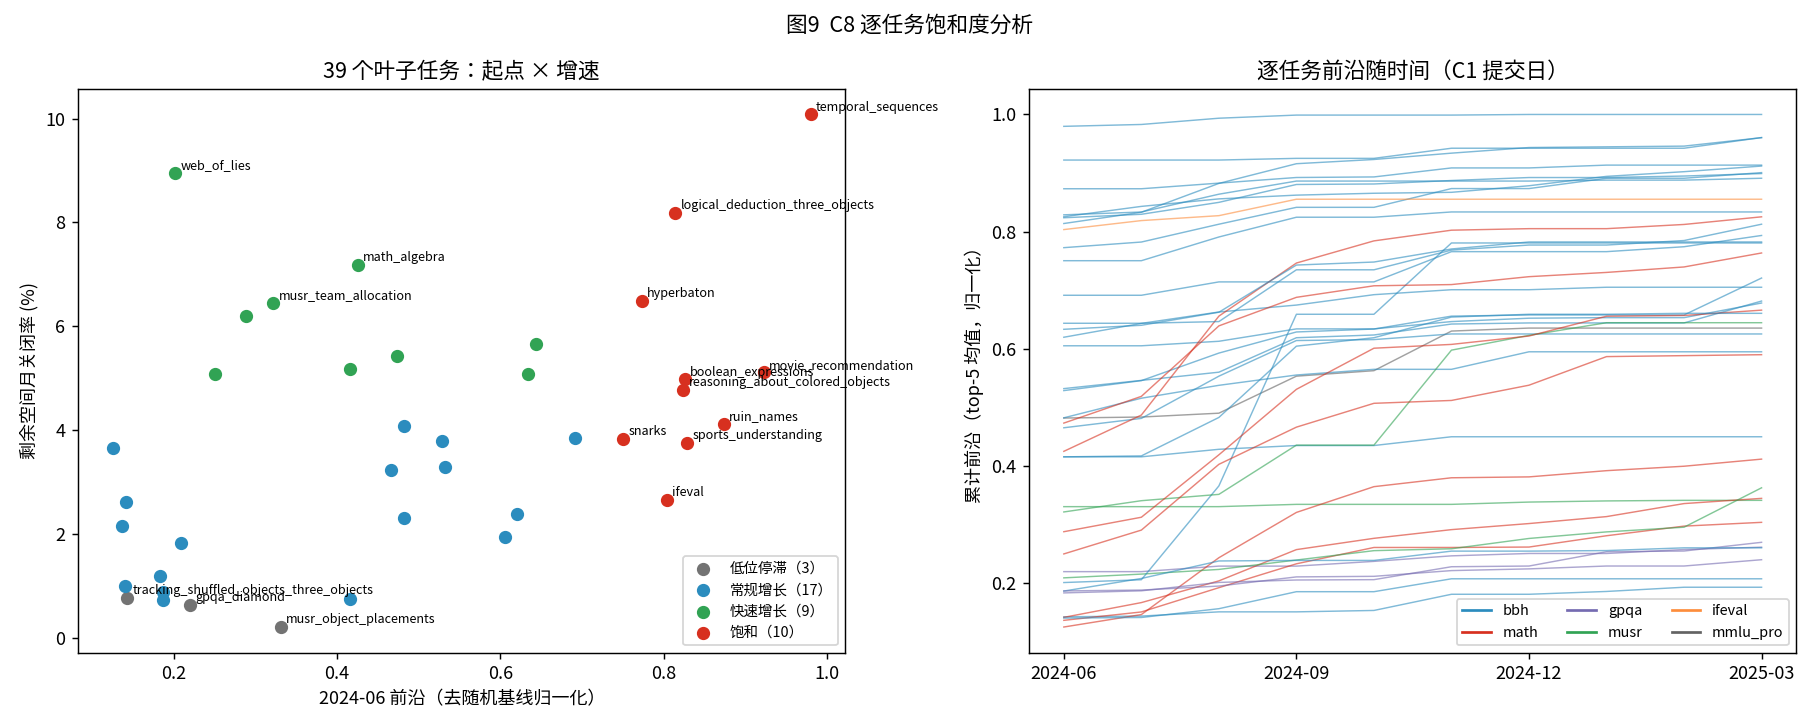
\includegraphics[width=\textwidth]{figs/q4_F9_task_saturation.png}
\caption{39 个叶子任务的饱和度分类}
\label{fig:F9_task_saturation}
\end{figure}

\begin{table}[H]
\centering\footnotesize
\caption{三种能力口径下的前沿变化（C1 提交日窗口 2024-06～2025-03；源自 \texttt{T5\_desat\_vs\_average.csv}，正文表格）}
\label{tab:q4desat}
\begin{tabularx}{\textwidth}{@{}X r r r r@{}}
\toprule
口径 & 起点前沿 & 终点前沿 & 相对增幅 & 月斜率 \\
\midrule
C1 \texttt{Average } & 38.52 & 49.89 & +29.53\% & 1.285 \\
C8 全任务重算 & 37.98 & 49.40 & +30.08\% & 1.326 \\
C8 去饱和分 & 26.36 & 39.06 & \textbf{+48.19\%} & 1.536 \\
\bottomrule
\end{tabularx}
\end{table}

表中相对增幅的分母为该口径的起点前沿。模型级去饱和分与 \texttt{Average} 的相关系数为 $0.9479$（\texttt{T5\_model\_desat\_scores.csv}，图~\ref{fig:F10_desat_vs_avg}），即两者排序基本一致，但按相对增幅计，包含饱和任务的 \texttt{Average} 低估前沿进展约 1.6 倍。图~\ref{fig:F10_desat_vs_avg} 的两个面板分别显示三个口径的归一化前沿与模型级散点。C8 重算与 C1 榜单的一致性核对（\texttt{T5\_c8\_vs\_c1\_check.csv}）为：五个任务族的 Pearson 在 $0.9893$–$0.9995$、MAE 在 $0.049$–$0.243$，\textbf{例外是 MATH（Pearson $0.8009$、MAE $3.4974$）}；这是同批评测数据的重算一致性核对，不是独立检验，MATH 例外的原因尚未解释。

\begin{figure}[H]
\centering
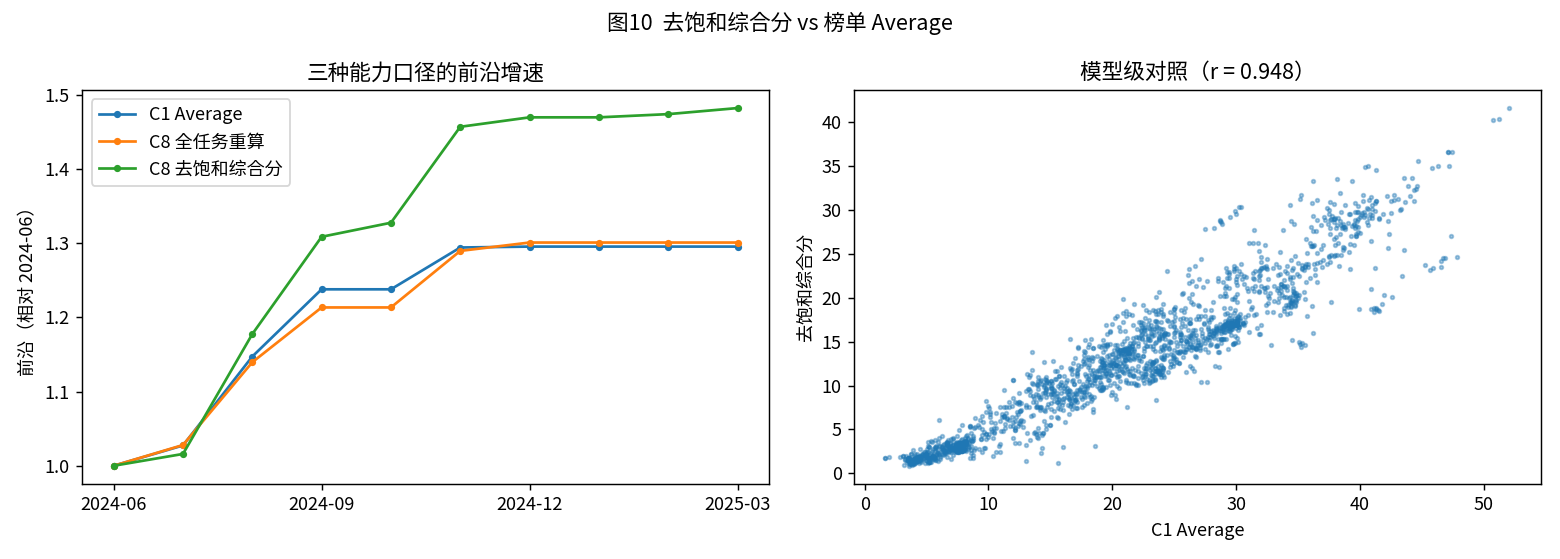
\includegraphics[width=\textwidth]{figs/q4_F10_desat_vs_avg.png}
\caption{去饱和综合分与 \texttt{Average} 口径的前沿对比}
\label{fig:F10_desat_vs_avg}
\end{figure}

\textbf{损失到得分的分层桥接。} C6 共 75 行，High 层 7 行、Medium 层 68 行。主桥接 \texttt{base|Average}（44 行）的参数为 $lo=8.626$、$hi=21.572$、$k=46.12$、$L_0=2.07$；\texttt{chat|Average}（31 行）为 $lo=12.096$、$hi=35.112$、$k=13.857$、$L_0=2.155$（\texttt{T6\_bridge\_fits.csv}、\texttt{interface/P4\_bridge\_params.json}，图~\ref{fig:F11_bridge}）。C6 全体的 Loss 与 \texttt{Average} 相关系数为 $-0.510$（High $-0.397$、Medium $-0.502$），符号为负，与"损失越低、得分越高"的方向一致。留一 RMSE 为 S 形 $8.079$、线性 $8.283$、常数 $9.514$，即 S 形略优于线性与常数（\texttt{T6\_bridge\_loo.csv}）。系列内固定效应斜率为 base $-23.58$、chat $-36.65$。Medium 层权重取 $0.25/0.5/1.0$ 时，$S(1.85)$ 分别为 $21.79/21.57/21.43$，结果稳定；仅用 High 层时只能得到 $lo=5.448$、$hi=6.349$，因为 High 层 7 点的损失全部落在 $[2.09,2.60]$ 的底噪区、对应得分仅 $5.1$–$6.1$（\texttt{T6\_bridge\_tier\_sensitivity.csv}）。因此\textbf{只能锁定下界 $lo$，S 形的上升段依赖 Medium 层}，这是 C6 数据的硬限制；表中的 $hi=21.572$ 是 C6 样本上拟合出的上平台，\textbf{不是榜单或未来能力的硬上限}。

\begin{figure}[H]
\centering
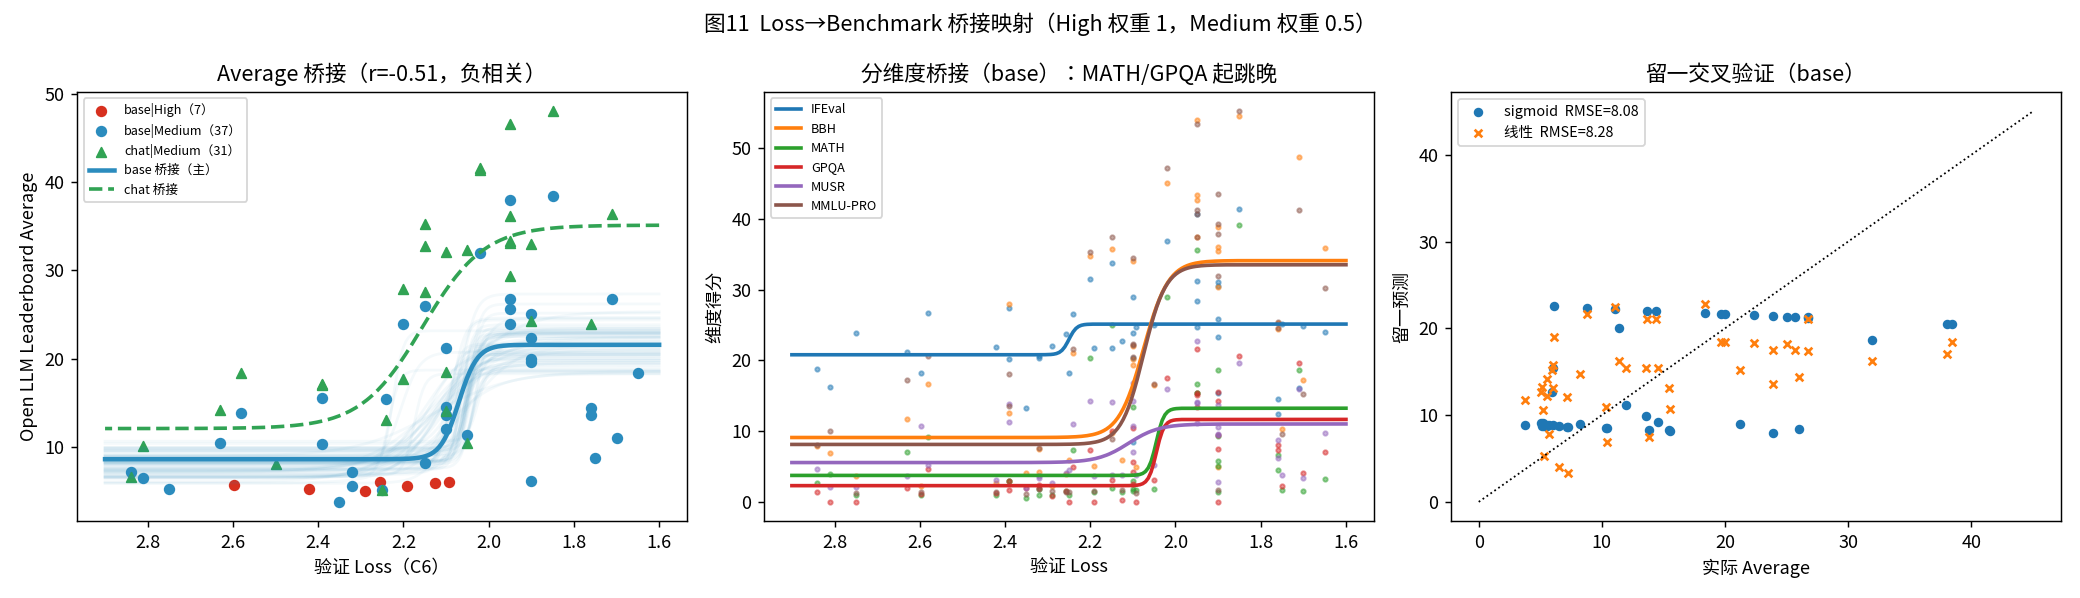
\includegraphics[width=\textwidth]{figs/q4_F11_bridge.png}
\caption{C6 分层 Loss–Benchmark 桥接（base 与 chat）}
\label{fig:F11_bridge}
\end{figure}

\textbf{规模与非规模贡献的分解。} 面板由 C2 与 C4 按（发布日期，组织）连接得到：base 58 行、chat 37 行；base 的 58 行中 35 行的 $D$ 来自 C4 数据量、23 行由 $C/(6N)$ 反解得到（后者是近似反解，不是实测数据量）。拟合优度为 M1b $R^2=0.8701$、M1c $0.8684$、仅规模重估 $0.8320$、OLS $0.6603$、M1a $0.5603$（\texttt{T7\_decomp\_fit\_quality.csv}）。主模型参数为 $\tau=2.4526$ 分/年（M1c 的 $\delta=0.035$ nats/年）。

\begin{table}[H]
\centering\footnotesize
\caption{base 前沿增长的贡献分解（窗口 2023.50$\to$2025.00，观测变化 $\Delta S_{\rm obs}=24.759$；源自 \texttt{interface/P4\_decomposition.csv}，正文表格）}
\label{tab:q4decomp}
\begin{tabularx}{\textwidth}{@{}l X r r r r r@{}}
\toprule
类别 & 方法 & 规模贡献 & 技术贡献 & 模型变化 & 技术占比 & 90\% 区间 \\
\midrule
结构模型 & \textbf{M1b（主）} & 23.063 & 3.404 & 26.467 & \textbf{12.86\%} & 6.07\%–21.96\% \\
结构模型 & M1c & 20.115 & 6.037 & 26.153 & 23.09\% & 4.17\%–45.49\% \\
线性对照 & M2 效率前沿 & 7.358 & 6.186 & 13.544 & 45.67\% & 8.68\%–59.88\% \\
线性对照 & M3 $q=0.75$ & 7.398 & 4.445 & 11.844 & 37.53\% & -47.38\%–58.24\% \\
线性对照 & M3 $q=0.90$ & 10.186 & -3.149 & 7.037 & -44.75\% & 跨零 \\
线性对照 & M3 $q=0.50$ & 6.241 & 5.875 & 12.116 & 48.49\% & 9.15\%–62.50\% \\
线性对照 & OLS & 7.722 & 3.235 & 10.957 & 29.53\% & 10.94\%–46.13\% \\
反例 & M1a（直接套用 C6 桥接） & 0.632 & 4.835 & 5.467 & 88.44\% & 80.04\%–92.08\% \\
\bottomrule
\end{tabularx}
\end{table}

\textbf{表中技术占比的分母是各方法自身的模型变化 $\Delta S_{\rm model}$，不是观测增量 $\Delta S_{\rm obs}$}；观测增量与模型增量并不闭合（base 为 $24.759$ 对 $26.467$），残差未分配，故这些百分比只能表述为"模型解释增量内部的份额"。图~\ref{fig:F12_decomp_panel} 显示面板中规模状态 $\hat L$、得分与时间的关系以及 M1b 在不同时间的曲线，图~\ref{fig:F13_decomp_bars} 给出各方法、各窗口的规模与技术贡献对比（含 8 个方法的技术占比标注与观测增量参考线）。核心三法（M1b、M2、M3 $q=0.75$）的技术占比极差为 $32.81$ 个百分点，方法分歧是结构性的：M2 与 M3 假设得分对 $\log_{10}C$ 线性，无法表达桥接的 S 形加速段，会把"损失刚进入陡峭区带来的规模红利"部分记入时间项；M1b/M1c 用"标度律＋S 形桥接"吸收这部分，拟合优度也明显更高（$0.87$ 对 $0.66$）。因此本文保留方法分歧，不给出唯一数字：结构口径的技术占比为 $12.9\%$–$23.1\%$（主口径 $12.9\%$），线性口径的 $29.5\%$–$48.5\%$ 作为上界参考；所有方法在"规模扩张为主"这一定性结论上一致。M1a 直接套用 C6 桥接（其 $hi=21.572$ 低于面板前沿 $37.302$），把桥接的非线性全部记入"技术"，得到 $88.4\%$，与索洛余值法的偏差同源，仅作反例。

\begin{figure}[H]
\centering
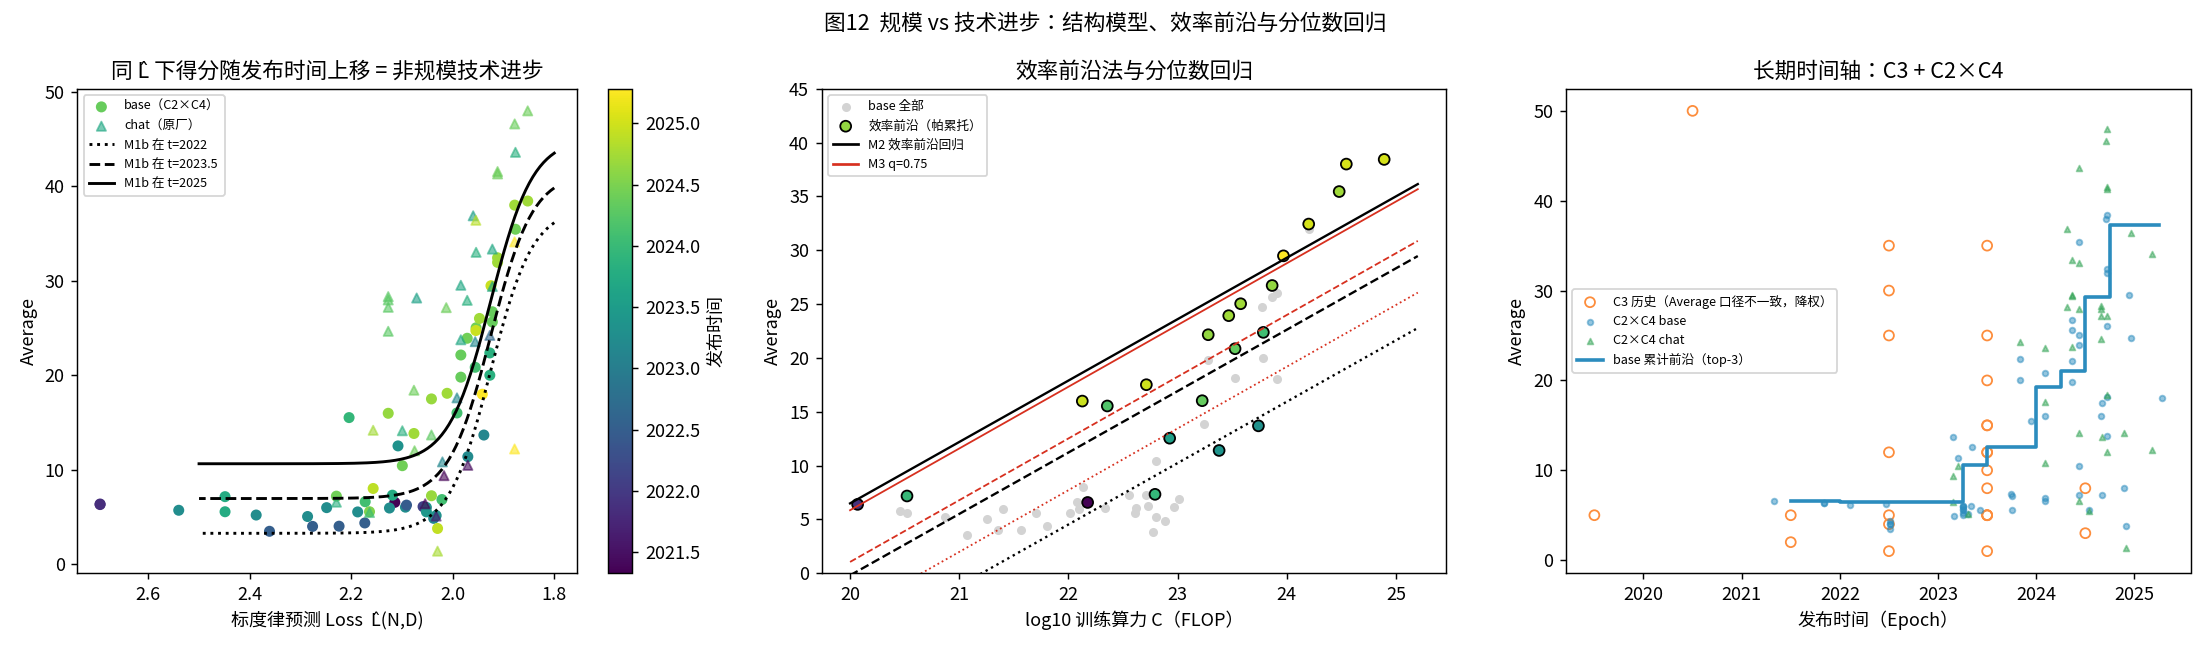
\includegraphics[width=\textwidth]{figs/q4_F12_decomp_panel.png}
\caption{分解面板：规模状态 $\hat L$、得分与时间}
\label{fig:F12_decomp_panel}
\end{figure}

\begin{figure}[H]
\centering
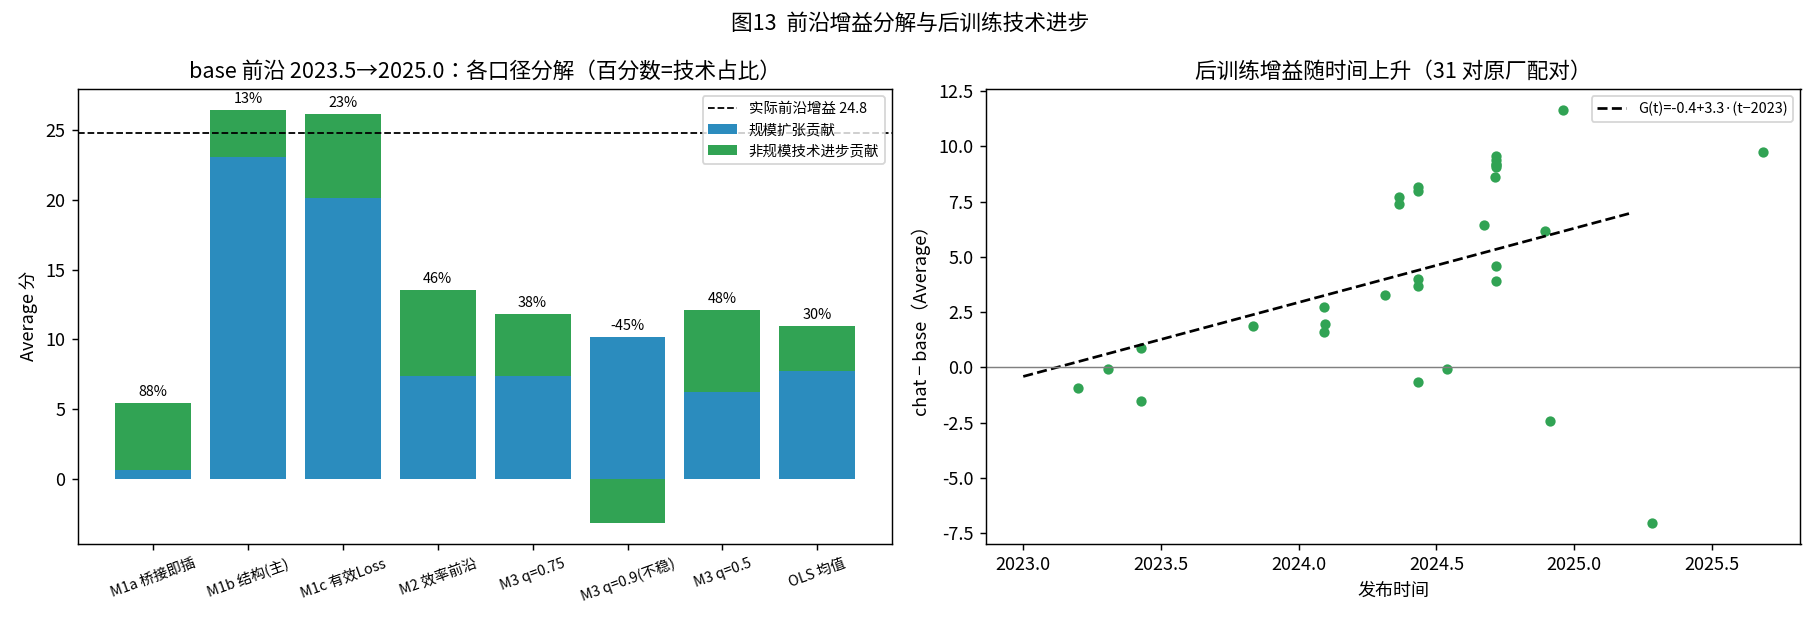
\includegraphics[width=\textwidth]{figs/q4_F13_decomp_bars.png}
\caption{各方法、各窗口的规模贡献与技术贡献}
\label{fig:F13_decomp_bars}
\end{figure}

窗口敏感性：换用 2024.00$\to$2025.00 时 M1b 的技术占比为 $7.06\%$；换用 2024.50$\to$2025.25 时为 $8.18\%$（M1a 在该窗口为 $99.30\%$，M3 $q=0.90$ 为负）。换算为算力等效速率，各方法的技术进步为 M1b $0.290$、M1c $0.561$、M2 $0.781$、M3 $q=0.75$ $0.558$、M3 $q=0.50$ $0.875$、OLS $0.389$ dex/yr（M3 $q=0.90$ 为 $-0.287$）（\texttt{T7\_compute\_equiv\_rate.csv}）。C3 历史点的降权敏感性：仅用 C2$\times$C4 时为 $0.781$ dex/yr（$n=58$），加入 C3 历史点、权重 $0.2$ 时为 $0.499$、权重 $1.0$ 时为 $0.205$（\texttt{T7\_c3\_sensitivity.csv}）。C3 的 \texttt{Average} 与其六维均值的相关仅为 $0.6337$，口径混杂，故\textbf{只作有标记的敏感性、不并入主面板}。C1 九个月窗口的短窗回归（同一批数据，非留出）给出 base 的月度等效 $0.722$ dex/yr（\texttt{Average} 口径）/ $0.766$（去饱和口径）与 chat 的 $0.444/0.572$，与上述量级一致（\texttt{T7\_c1\_window\_check.csv}）。

chat 与后训练：在 89 对同组织的 (base, chat) 配对中平均增益为 $4.304$ 分、中位数 $3.696$ 分；对有发布日的 31 对回归得 $G(t)=-0.405+3.348(t-2023)$，说明后训练本身是一类逐年增强的非规模技术（\texttt{T7\_chat\_posttrain\_pairs.csv}）。chat 前沿在 2023.50$\to$2025.00 由 $8.76$ 升至 $46.06$（观测增量 $37.293$），其中规模贡献 $23.766$、预训练技术 $3.563$、后训练技术 $4.863$，模型变化合计 $32.191$、技术占比 $26.17\%$（\texttt{T7\_chat\_decomposition.csv}）。chat 同样\textbf{须报告观测增量与模型增量的不闭合}。

\textbf{算力情景与前沿预测。} C4 中开放权重模型的年度训练算力：2025 年有 112 个点（\texttt{open\_max\_log10C} 为 $25.592$、Top-5 均值为 $25.049$）；斜率按不同统计口径为 $0.579$（open\_max，2019–2025）、$0.598$（open\_top5）、$0.688$（open\_max，2022–2025）、$0.646$（all\_max）dex/yr（\texttt{T8\_compute\_trend.csv}）。据此设三种情景：基线 $0.60$、减半 $0.30$、四分之一 $0.15$ dex/yr。起点 $T_0=2025.25$，锚点 base $S=37.302$、chat $S=46.057$，12/24 个月的目标日期为 2026.25/2027.25。

\begin{table}[H]
\centering\footnotesize
\caption{开源前沿（\texttt{Average}）的条件情景外推：中位数 [5\%–95\% 区间]（数据源：\texttt{interface/P4\_frontier\_forecast.csv}）}
\label{tab:q4fc}
\begin{tabularx}{\textwidth}{@{}l c c c X X@{}}
\toprule
情景 & \makecell{base\\12 个月} & \makecell{base\\24 个月} & \makecell{base 24 个月\\技术占比} & \makecell{chat 24 个月\\（后训练延续）} & \makecell{chat 24 个月\\（后训练停滞）} \\
\midrule
基线 0.60 & 43.07\,[37.35, 52.83] & 46.19\,[37.55, 68.49] & 54.94\% & 61.62\,[51.79, 79.62] & 54.85\,[46.43, 70.12] \\
减半 0.30 & 41.73\,[36.95, 49.66] & 45.25\,[37.75, 58.28] & 65.49\% & — & — \\
四分之一 0.15 & 41.09\,[36.63, 47.59] & 44.11\,[37.53, 54.86] & 76.70\% & — & — \\
\bottomrule
\end{tabularx}
\end{table}

算力增速从 $0.60$ 降到 $0.15$ dex/yr，24 个月的 base 中位数只减少约 2 分（$46.19\to44.11$）：规模增量本身被 S 形桥接的饱和段压缩，而技术项基本不受算力情景影响，因此\textbf{算力放缓时技术进步成为增量主体}（24 个月技术占比由 $54.94\%$ 升至 $76.70\%$）。图~\ref{fig:F14_forecast} 的左、中面板给出三情景下 base/chat 的区间扇形与 M1b 的纯规模天花板（$44.195$），右面板给出回测误差。模型不确定性主要来自技术项形式：基线情景下 24 个月的 M1b 中位数为 $46.590$、M1c 为 $44.719$；chat 对"后训练增益是否延续"最敏感（$61.62$ 对 $54.85$，相差约 6.8 分），这一差别大于算力情景之间的差别（约 2 分）。作为上界参考，"算力无限"时 24 个月的 M1b 为 $49.177$（\texttt{T8\_forecast\_by\_techform.csv}，\texttt{T8\_forecast\_meta.json} 的 \texttt{caps}）。预测区间只包含问题二参数、分解簇 bootstrap、后训练增益与面板残差，\textbf{不包含 C6 桥接的迁移误差}；另有累计前沿区间下界在部分情景低于锚点（如减半情景 12 个月 base 的 5\% 分位为 $36.95$、低于锚点 $37.302$），与"累计前沿不下降"的定义冲突，须按"当期新模型前沿"重新定义或修正模拟。

\begin{figure}[H]
\centering
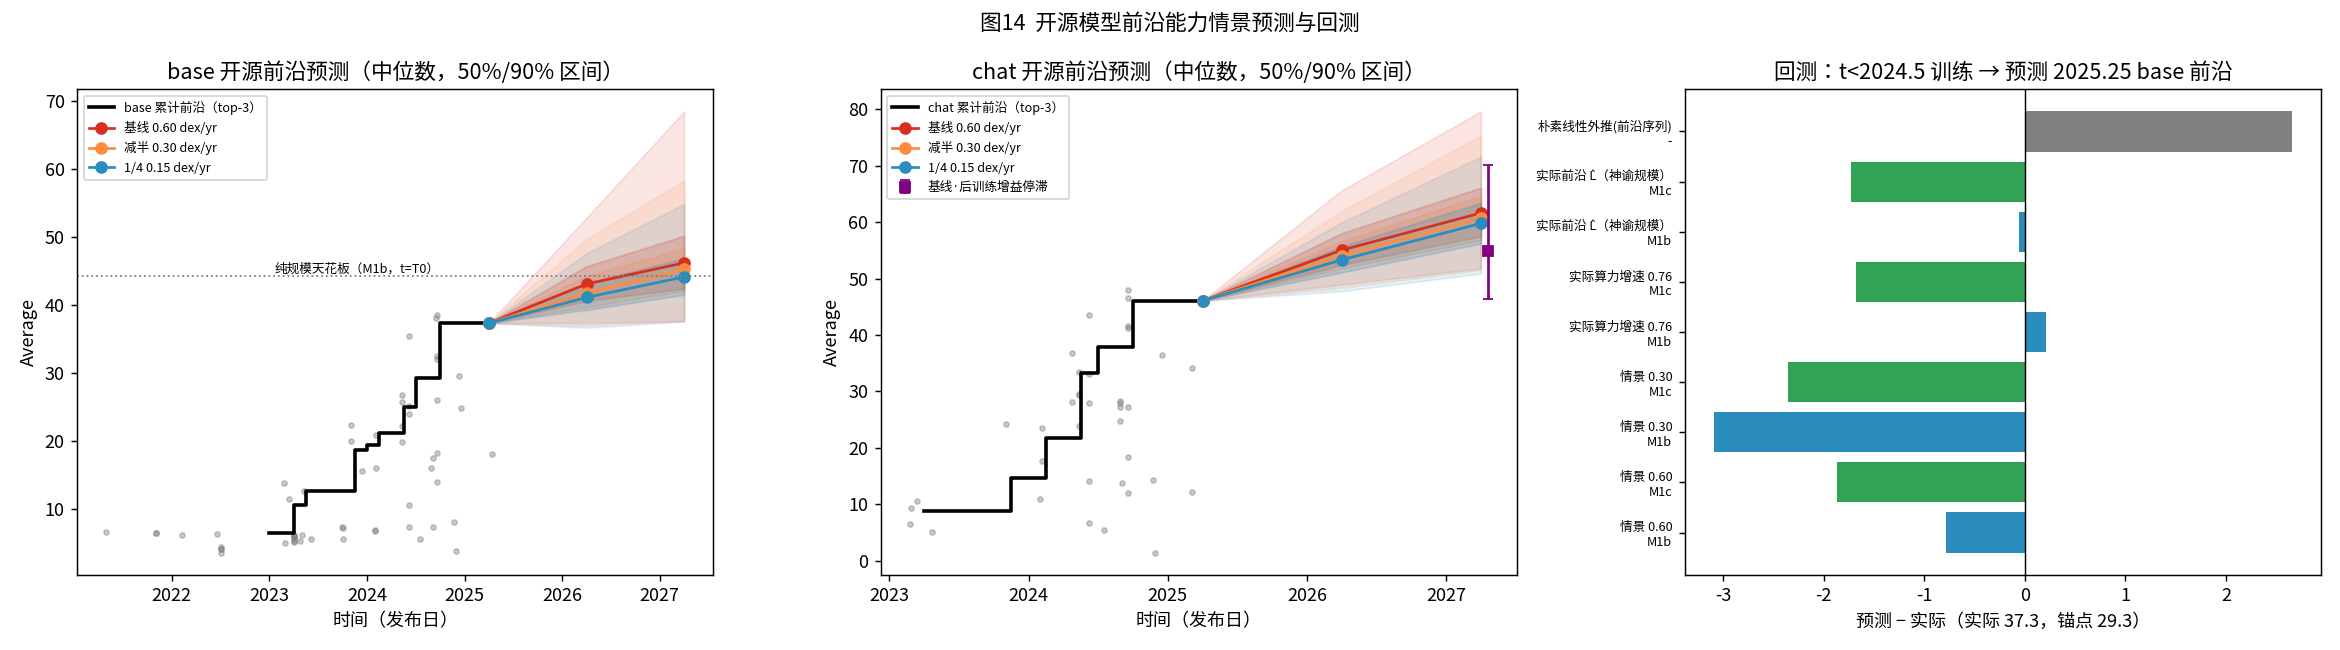
\includegraphics[width=\textwidth]{figs/q4_F14_forecast.png}
\caption{三种算力情景下 base/chat 前沿的条件外推}
\label{fig:F14_forecast}
\end{figure}

\textbf{回测。} 在发布日轴上只用 $t<2024.5$ 的 42 个 base 模型重估模型（$\tau=2.741$），以 2024.5 的前沿 $29.277$ 为锚点预测 2025.25 的实际前沿 $37.302$：基线情景 M1b 的误差为 $-0.784$、M1c 为 $-1.867$；用实际算力增速 $0.758$ dex/yr 时 M1b 误差为 $+0.212$；用实际前沿的规模状态（神谕规模）时 M1b 误差为 $-0.054$；朴素线性外推的误差为 $+2.651$（\texttt{T8\_backtest.csv}）。在提交日轴上，对 C1 月度前沿做纯时间序列外推，3 个月误差达到 $+7.907$，因为前沿已在 $49.891$ 附近进入平台，这是不直接用 ARIMA 类外推的实证理由。回测的重估样本并非严格的起点前冻结样本（见本节开头限制），故只能称"事后回测表现"，不能称独立预测验证。
